\documentclass[tikz,border=6pt]{standalone}
\usepackage{tikz}
\usetikzlibrary{arrows.meta,calc}
\begin{document}
\sffamily
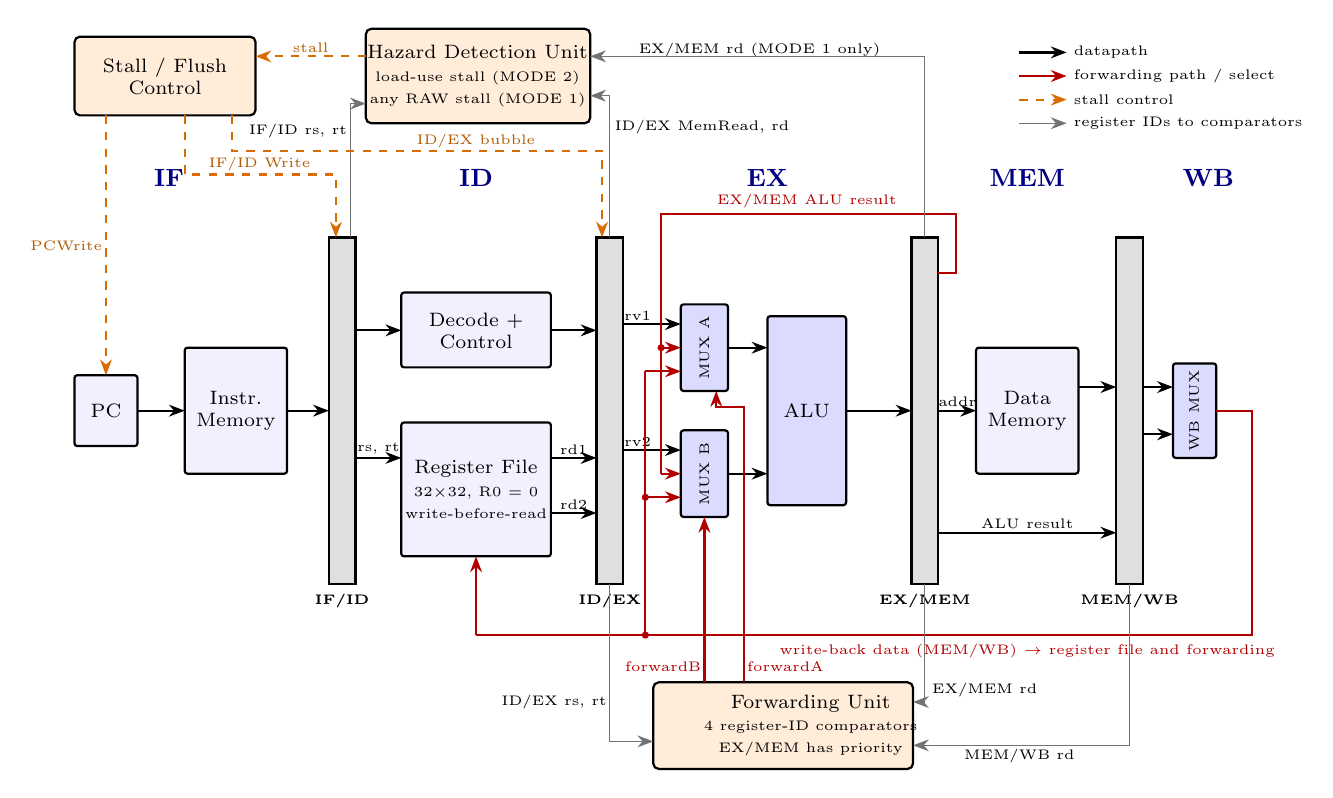
\begin{tikzpicture}[
  >={Stealth[length=2mm]}, font=\scriptsize,
  blk/.style={draw, thick, fill=blue!6, align=center, rounded corners=1pt},
  ctl/.style={draw, thick, fill=orange!15, align=center, rounded corners=2pt},
  preg/.style={draw, thick, fill=gray!25},
  dp/.style={->, thick},
  fw/.style={->, thick, red!70!black},
  hz/.style={->, thick, orange!85!black, dashed},
  info/.style={->, thin, black!55},
  lab/.style={font=\tiny, inner sep=1pt}
]
% ---------- stage titles ----------
\foreach \x/\t in {0.8/IF, 4.7/ID, 8.4/EX, 11.7/MEM, 14.0/WB}
  \node[font=\small\bfseries, text=blue!50!black] at (\x,2.95) {\t};
% ---------- pipeline registers ----------
\foreach \x/\n/\t in {3.0/r1/{IF/ID}, 6.4/r2/{ID/EX}, 10.4/r3/{EX/MEM}, 13.0/r4/{MEM/WB}} {
  \draw[preg] (\x-0.17,-2.2) rectangle (\x+0.17,2.2);
  \node[lab, font=\tiny\bfseries] at (\x,-2.42) {\t};
}
% ---------- IF ----------
\draw[blk] (-0.4,-0.45) rectangle (0.4,0.45); \node at (0,0) {PC};
\draw[blk] (1.0,-0.8) rectangle (2.3,0.8);   \node[align=center] at (1.65,0) {Instr.\\Memory};
\draw[dp] (0.4,0) -- (1.0,0);
\draw[dp] (2.3,0) -- (2.83,0);
% ---------- ID ----------
\draw[blk] (3.75,0.55) rectangle (5.65,1.5);   \node[align=center] at (4.7,1.02) {Decode +\\Control};
\draw[blk] (3.75,-1.85) rectangle (5.65,-0.15); \node[align=center] at (4.7,-1.0) {Register File\\{\tiny 32$\times$32, R0 = 0}\\{\tiny write-before-read}};
\draw[dp] (3.17,1.02) -- (3.75,1.02);
\draw[dp] (3.17,-0.6) -- node[lab, above]{rs, rt} (3.75,-0.6);
\draw[dp] (5.65,1.02) -- (6.23,1.02);
\draw[dp] (5.65,-0.6) -- node[lab, above]{rd1} (6.23,-0.6);
\draw[dp] (5.65,-1.3) -- node[lab, above]{rd2} (6.23,-1.3);
% ---------- EX ----------
\draw[blk, fill=blue!14] (7.3,0.25) rectangle (7.9,1.35);   \node[lab, rotate=90] at (7.6,0.8) {MUX A};
\draw[blk, fill=blue!14] (7.3,-1.35) rectangle (7.9,-0.25); \node[lab, rotate=90] at (7.6,-0.8) {MUX B};
\draw[blk, fill=blue!14] (8.4,-1.2) rectangle (9.4,1.2);   \node at (8.9,0) {ALU};
\draw[dp] (6.57,1.1) -- node[lab, above, pos=0.25]{rv1} (7.3,1.1);
\draw[dp] (6.57,-0.5) -- node[lab, above, pos=0.25]{rv2} (7.3,-0.5);
\draw[dp] (7.9,0.8) -- (8.4,0.8);
\draw[dp] (7.9,-0.8) -- (8.4,-0.8);
\draw[dp] (9.4,0) -- (10.23,0);
% ---------- MEM ----------
\draw[blk] (11.05,-0.8) rectangle (12.35,0.8); \node[align=center] at (11.7,0) {Data\\Memory};
\draw[dp] (10.57,0) -- node[lab, above]{addr} (11.05,0);
\draw[dp] (12.35,0.3) -- (12.83,0.3);
\draw[dp] (10.57,-1.55) -- node[lab, above]{ALU result} (12.83,-1.55);
% ---------- WB ----------
\draw[blk, fill=blue!14] (13.55,-0.6) rectangle (14.1,0.6); \node[lab, rotate=90] at (13.82,0) {WB MUX};
\draw[dp] (13.17,0.3) -- (13.55,0.3);
\draw[dp] (13.17,-0.3) -- (13.55,-0.3);
% write-back bus: WB mux -> register file, also the MEM/WB forwarding source
\draw[thick, red!70!black] (14.1,0) -- (14.55,0) -- (14.55,-2.85) -- (4.7,-2.85);
\draw[dp, red!70!black] (4.7,-2.85) -- (4.7,-1.85);
\node[lab, text=red!70!black] at (11.7,-3.05) {write-back data (MEM/WB) $\rightarrow$ register file and forwarding};
% ---------- forwarding paths ----------
% EX/MEM result lane
\draw[thick, red!70!black] (10.57,1.75) -- (10.8,1.75) -- (10.8,2.5) -- (7.05,2.5) -- (7.05,-0.8);
\node[lab, text=red!70!black] at (8.9,2.66) {EX/MEM ALU result};
\draw[fw] (7.05,0.8) -- (7.3,0.8);
\draw[fw] (7.05,-0.8) -- (7.3,-0.8);
\fill[red!70!black] (7.05,0.8) circle (1.3pt);
% MEM/WB lane
\draw[thick, red!70!black] (6.85,-2.85) -- (6.85,0.5);
\fill[red!70!black] (6.85,-2.85) circle (1.3pt);
\fill[red!70!black] (6.85,-1.1) circle (1.3pt);
\draw[fw] (6.85,0.5) -- (7.3,0.5);
\draw[fw] (6.85,-1.1) -- (7.3,-1.1);
% ---------- forwarding unit ----------
\draw[ctl] (6.95,-4.55) rectangle (10.25,-3.45);
\node[align=center] at (8.95,-4.0) {Forwarding Unit\\{\tiny 4 register-ID comparators}\\{\tiny EX/MEM has priority}};
\draw[fw] (7.6,-3.45) -- (7.6,-1.35);
\node[lab, text=red!70!black, left] at (7.6,-3.25) {forwardB};
\draw[fw] (8.1,-3.45) -- (8.1,0.05) -- (7.75,0.05) -- node[lab, right, pos=0.0]{} (7.75,0.25);
\node[lab, text=red!70!black, right] at (8.1,-3.25) {forwardA};
\draw[info] (6.4,-2.2) -- (6.4,-4.2) -- (6.95,-4.2);
\node[lab, left] at (6.4,-3.7) {ID/EX rs, rt};
\draw[info] (10.4,-2.2) -- (10.4,-3.7) -- (10.25,-3.7);
\draw[info] (13.0,-2.2) -- (13.0,-4.25) -- (10.25,-4.25);
\node[lab, right] at (10.45,-3.55) {EX/MEM rd};
\node[lab, below] at (11.6,-4.25) {MEM/WB rd};
% ---------- hazard detection + stall/flush control ----------
\draw[ctl] (3.3,3.65) rectangle (6.15,4.85);
\node[align=center] at (4.72,4.25) {Hazard Detection Unit\\{\tiny load-use stall (MODE 2)}\\{\tiny any RAW stall (MODE 1)}};
\draw[ctl] (-0.4,3.75) rectangle (1.9,4.75);
\node[align=center] at (0.75,4.25) {Stall / Flush\\Control};
\draw[info] (3.1,2.2) -- (3.1,3.9) -- (3.3,3.9);
\node[lab, left] at (3.1,3.55) {IF/ID rs, rt};
\draw[info] (6.4,2.2) -- (6.4,4.0) -- (6.15,4.0);
\node[lab, right] at (6.42,3.6) {ID/EX MemRead, rd};
\draw[info] (10.4,2.2) -- (10.4,4.5) -- (6.15,4.5);
\node[lab, above] at (8.3,4.45) {EX/MEM rd (MODE 1 only)};
\draw[hz] (3.3,4.5) -- node[lab, above, text=orange!70!black]{stall} (1.9,4.5);
\draw[hz] (0.0,3.75) -- node[lab, left, text=orange!70!black]{PCWrite} (0.0,0.45);
\draw[hz] (1.0,3.75) -- (1.0,3.0) -- (2.92,3.0) -- (2.92,2.2);
\node[lab, text=orange!70!black, above] at (1.95,3.0) {IF/ID Write};
\draw[hz] (1.6,3.75) -- (1.6,3.3) -- (6.3,3.3) -- (6.3,2.2);
\node[lab, text=orange!70!black, above] at (4.7,3.3) {ID/EX bubble};
% ---------- legend ----------
\begin{scope}[shift={(11.6,4.55)}]
  \draw[dp] (0,0) -- (0.6,0);           \node[lab, right] at (0.65,0) {datapath};
  \draw[fw] (0,-0.3) -- (0.6,-0.3);     \node[lab, right] at (0.65,-0.3) {forwarding path / select};
  \draw[hz] (0,-0.6) -- (0.6,-0.6);     \node[lab, right] at (0.65,-0.6) {stall control};
  \draw[info] (0,-0.9) -- (0.6,-0.9);   \node[lab, right] at (0.65,-0.9) {register IDs to comparators};
\end{scope}
\end{tikzpicture}
\end{document}
